\section{Projet}
	
	
\def\slp{XXX }


% FL : balises de commentaires déplacées dans rapportEquipeSLP.tex


		\subsection{Analyse SWOT}
		 
		\restylefloat{table}
		 \renewcommand{\labelitemi}{$\bullet$}
		 

			\restylefloat{table}
			\begin{table}[H]
			\begin{tabularx}{\textwidth}{|>{\centering\arraybackslash}l|>{\centering\arraybackslash}X|>{\centering\arraybackslash}X|}
			\hline
			&\textcolor{red}{Positif (pour atteindre l'objectif)} & \textcolor{red}{Négatif (pour atteindre l'objectif)}\\
			\hline
			\color{red}\parbox[t]{2mm}{\rotatebox[origin=rB]{90}{ Origine Interne (organisationnelle) }} & \centering\textcolor{red}{Forces} 
			\smallskip
			\begin{itemize}
			% FORCES 
			\item  Recentrage des thématiques de recherche, ce qui resserre le champ de recherche de l'équipe et renforce la lisibilité de ses thèmes de recherche.
			\item Les thématiques de l'équipe se prêtent aussi bien à une recherche théorique qu'à une recherche appliquée. Les chercheurs passent naturellement de l'une à l'autre. 
			\item L'équipe à un fort niveau de publication, un bon volume de projet.
			\item IMT Atlantique a réinvesti des ressources humaines dans l'équipe.
			
			\end{itemize} ~\\ & \textcolor{red}{Faiblesses}
			\smallskip
			\begin{itemize}
			%FAIBLESSES
			
			\item L'équipe reste une grosse équipe avec une large couverture thématique, si bien qu'il est difficile de fédérer tous les chercheurs autour de projets communs.
			
			\end{itemize}\\
			\hline
			\centering\color{red}\parbox[t]{2mm}{\rotatebox[origin=rB]{90}{ Origine Interne (organisationnelle) }} & \centering\textcolor{red}{Opportunité} 
			\smallskip
			\begin{itemize} 
			% OPPORTUNITE
			\item  Les sujets de recherche de l'équipe sont au carrefour de plusieurs problématiques majeures, telle que la transition numérique, l'intelligence artificielle, les sciences des données. Notamment, la montée en puissance du numérique dans l'industrie, les services, les transports, rendent accessibles des données qui ne l'étaient pas auparavant. 
			\item L'industrie du futur, la mobilité des biens et personnes, la santé, font partie des verrous scientifiques majeurs de nombreux  appels à projet nationaux et européens.
			\item Dans le domaine de la santé, les aspects logistique et de planification seront peut-être examinés demain sous un aspect nouveau.
			\item  Plusieurs recrutements récents, qui apportent une nouvelle dynamique à l'équipe, et permettent de casser le cloisonnement antérieur de l'équipe en axes trop indépendants.
			\end{itemize} & \textcolor{red}{Menaces}
			\smallskip
			\begin{itemize} 
			\item  Départ de Philippe Castagliola et disparition de fait de l'axe Maîtrise des Risques pour les Systèmes Industriels et les Services. L'organisation de l'équipe doit donc être revue. Risque de baisse du niveau de publication. 
			\item Manque de visibilité de la discipline ``recherche opérationnelle" par rapport à la discipline beaucoup plus vaste de l'intelligence artificielle. Ce phénomène n'est pas nouveau. 
			\item  SLP est majoritairement basée à IMT Atlantique, qui n'est pas impliqué dans NExT. 
			Incertitudes sur l'avenir du paysage Nantais de la recherche. 
			\end{itemize}\\
			\hline
			\end{tabularx}
			\end{table}
		 

		\subsection{Structuration, effectifs et orientations scientifiques}
		
		\OP{Il y a des parties plus ou moins bien rédigées, ce qui n'empêche pas de réagir sur le fond}
		

\textcolor{blue}{Pour l’unité, (l’équipe / le thème), on précisera le mode de structuration et on présentera les effectifs, les orientations scientifiques, les choix stratégiques, les objectifs scientifiques, les moyens à mobiliser pour atteindre ces objectifs, les partenariats, les nouvelles thématiques scientifiques, etc.
Pour rédiger cette partie, on prendra soin de commenter les objectifs et réalisations attendues contenues dans l’onglet 3 du fichier Excel « Données du prochain contrat ».}



\subsubsection{Contexte}
		
		Les thèmes de recherche de l'équipe peuvent s'inscrire dans le cadre beaucoup plus général de la transition numérique. 
		L'accélération des cycles de vie des produits rend nécessaire la mise en place de systèmes de production et des système logistiques flexibles, reconfigurables tout en restant performants. 
		Même dans un univers changeant, certaines décision doivent être prises pour du long terme. 
		Cette confrontation entre l'horizon stratégique et les décisions opérationnelles renforce l'intérêt de concevoir des systèmes adaptables. 
		Le projet d'équipe voit donc monter en puissance la thématique de l'optimisation dans l'incertain \OP{au sens TRES large}. 
		Il s'agit de prendre en compte l'incertitude des données, le risque lié à certaines décisions, allant de simples aléas 	jusqu'aux risques systémiques. 
		
		Par ailleurs, l'irruption de la donnée massive dans tous les champs de l'économie rend possible des projets de recherche et d'innovation qui ne l'étaient pas il y a quelques années. 
		Cette transition numérique modifie de nombreux modèles d'entreprise (servicisation, pratiques collaboratives, mutualisation de moyens), ce qui fait évoluer les modèles traditionnels d'optimisation industrielle. 
		Le contexte actuel offre donc à l'équipe de nombreuses opportunités de développer son activité. 


	Contexte équipe : 
			
		\begin{itemize}
			\item Départ de Casta, disparition de son axe
			\item Nouvelle présentation de l'équipe, on abandonne les axes traditionnels
			\item Organisation selon 3 verrous scientifiques 
			\item Déclinés en objectifs de contribution
			\item pour répondre à des défis sociétaux majeurs
			\item avec des domaines d'application dans les systèmes de production, les chaines logistiques, le transport, les services
			\item L'activité de chaque membre de l'équipe s'inscrit dans un ou plusieurs défis sociétaux, verrous, objectifs et domaines d'application. 
		\end{itemize}
		
		L'équipe SLP (Systèmes Logistiques et de Production) change donc de nom et devient l'équipe \slp. \OP{A compléter}
		
		
		
		\subsubsection{Evolution des thématiques de recherche}
		
		Les thématiques de recherche de l'équipe \slp sont synthétisées par la Figure \ref{fig:projet}. 
		L'équipe se présente comme une équipe de recherche opérationnelle visant à résoudre des problèmes d'optimisation qui surviennent dans le cadre très vaste de la transition numérique.
		Elle n'a plus d'activité dans le domaine de la maitrise statistique des procédés et de la fiabilité, mais souhaite renforcer la thématique de l'optimisation dans l'incertain.
		
 
	Le projet de recherche s'articule autour de trois verrous scientifiques et techniques. Le premier vise à développer des méthodes de résolution de problèmes d'\textit{optimisation combinatoire}. Il constitue l'ADN de l'équipe \slp, dans la mesure où tous ses membres y contribuent. 
	Le deuxième se concentre sur des problèmes d'\textit{optimisation dans l'incertain}.
	Cette thématique gagne en visibilité dans ce nouveau projet.
	Le troisième introduit la prise en compte des \textit{contraintes et préférences complexes}, avec l'objectif de formuler et résoudre des problèmes d'optimisation qui reflètent aussi fidèlement que possible les modes de fonctionnement des utilisateurs finaux et tiennent compte des pratiques émergentes dans les domaines étudiés.
	Le premier verrou était déjà présent depuis la création de l'équipe SLP, les deux derniers sont nouveaux et témoignent d'un élargissement des compétences de l'équipe.
	
	Pour chacun de ces trois verrous, la Figure \ref{fig:projet} comporte deux colonnes. La colonne de gauche décline le verrou scientifique en plusieurs disciplines relevant de la recherche opérationnelle. La colonne de droite liste des caractéristiques de problèmes d'optimisation qui se posent dans le contexte de l'industrie du futur. Cette présentation illustre le fait que chaque verrou scientifique peut être abordé sous le prisme de contributions théoriques ou appliquées. 
	
	
	\subsubsection*{Verrou \# 1 : optimisation combinatoire}
	
	De par ses domaines d'application, l'équipe travaille essentiellement dans le domaine de l'optimisation combinatoire (également appelée optimisation discrète). De nombreux problèmes d'optimisation possèdent conjointement deux types de variables : des variables discrètes et des variables continues. On parle alors de problèmes mixtes. La plupart de ces problèmes d'optimisation ont de manière évidente une complexité non polynomiale. Dans l'étude des systèmes de production, notamment en ordonnancement, la complexité des problèmes étudiés reste parfois à prouver et fait l'objet d'études de complexité. Les méthodes de résolution abordées par l'équipe concernent aussi bien le développement de méthodes exactes (génération de colonnes, énumération implicite des solutions, algorithmes ad hoc) et de méthodes approchées (heuristiques, métaheuristiques et matheuristiques). 
	%
	L'équipe continuera son activité de mise en {\oe}uvre de méthodes exactes et de méthodes approchées. Elle développera la recherche de méthodes dites matheuristiques, c'est-à-dire hybridant méthodes exactes et approchées, de manière à conjuguer les avantages des deux approches (obtenir des solutions quasi optimales en un temps de calcul maîtrisé).
	
	Un dernier domaine de recherche est la mise au point d'algorithmes de basse complexité pour des problèmes polynomiaux. Ces algorithmes peuvent avoir un grand intérêt lorsqu'ils sont appelés à un nombre très grand de reprises par un autre algorithme. Cela peut concerner par exemple des tests de faisabilité d'une solution, des tests d'insertion d'un élément dans une solution, etc.
	
	Les principales applications visées par ces travaux concernent les problèmes d'optimisation dans les systèmes dits intégrés, c'est-à-dire comportant plusieurs niveaux de décisions (par exemple problèmes joints de planification et ordonnancement, de localisation et de routage, problèmes de planification de tâches et de personnel). Un autre champ d'application concerne les systèmes multi-échelons, 
	dans lesquels les processus étudiés comportent plusieurs phases successives (problème de production sur plusieurs ateliers, plusieurs phases de production, réseaux logistiques complexes ou hiérarchisés). 
	Pour l'ensemble de ces exemples, les méthodes de résolution nécessitent en effet de décomposer le problème initial en plusieurs sous-problèmes, qui seront résolus indépendamment soit de manière exacte soit de manière heuristique.  Les méthodes de décomposition permettent d'identifier et traiter des sous-composantes plus ou moins indépendantes des problèmes à résoudre, ou d'agréger les données de manière à permettre un passage à l'échelle. 
	%
	La problématique de la taille des instances à traiter risque de devenir de plus en plus prégnante avec la possibilité de recueillir facilement d'importants volumes de données. 
	
	Enfin, l'équipe poursuivra ses travaux sur les systèmes avec contraintes de synchronisation entre acteurs, que ce soient des véhicules, des personnes ou des composantes d'un système de production. 
	
	
	\subsubsection*{Verrou \# 2 : optimisation dans l'incertain}
	
	\OP{Angle d'attaque pour cette section : aller de l'aléa mineur vers l'aléa majeur}
	
	La demande croissante de l'industrie pour une meilleure maîtrise des aléas dans ses processus motive aujourd'hui l'équipe à développer et approfondir son expertise dans le domaine de l'optimisation sous incertitudes. Les derniers recrutements ont été réalisés dans cette optique. 
	
	%Tout d'abord, le terme  de \textit{variabilité} \OP{mot bien choisi ? } renvoie aux situations dans lesquelles les données et paramètres d'un problème déterministe varient dans le temps, le problème concerné restant par ailleurs dans un univers déterministe. 
	Le terme {\em incertitude} peut renvoyer à différentes situations, dont la nature détermine la mise en oeuvre de méthodes spécifiques en fonction de leurs caractéristiques.
	Même des problèmes considérés comme déterministes peuvent intégrer des paramètres variables dans le temps, dont les données fluctuent ou apparaissent progressivement (nouvelle commande, ordre de fabrication non planifié, retard, no-show, etc). 
	Les décideurs doivent alors être en mesure de reconstruire dynamiquement une nouvelle solution en intégrant les données au fil de l'eau, sans remettre en cause l'intégralité des décisions prises auparavant.
%
	Le défi principal est donc de parvenir à ré-optimiser localement une solution existante, en un temps de calcul très court, sans perdre de vue la qualité globale de celle-ci. 
 	Il existe également des techniques d'optimisation en plusieurs étapes qui peuvent s'avérer pertinentes lorsque l'on connaît plusieurs scénarios possibles d'évolution des paramètres d'un problème. Celles-ci permettent notamment de garantir que les décisions prises à un instant donné sont cohérentes avec les différentes décisions futures possibles, déterminées après l'apparition de nouvelles informations, et optimisées en conséquence.
	
	
	En \textit{optimisation stochastique}, certaines données des problèmes étudiés sont représentées par des variables aléatoires. 
	Cela peut aussi bien concerner la demande de clients que les prix, les niveaux de productivité, les retards ou avances, etc. 
	Cette classe de problème permet donc de modéliser un grand nombre de situations réalistes, à partir du moment où on est capable de modéliser l'incertitude avec une précision suffisante. 
	Tous les domaines d'application des travaux de l'équipe se prêtent à l'utilisation de l'optimisation stochastique. On différenciera toutefois les applications pour lesquelles la source d'incertitude provient de facteurs purement techniques (temps de trajet, durée d'exécution, coûts, etc) des applications où l'incertitude résulte de facteurs humains. Dans le premier cas, la modélisation des phénomènes par une variable aléatoire permet de traiter le problème par l'optimisation stochastique. Dans le deuxième cas, des travaux pluridisciplinaires avec des chercheurs en sciences de l'homme \GM{humaines?}  seront envisagés. \OP{Odile ? }
	
	
	L'\textit{optimisation robuste} consiste à construire des solution qui restent efficaces \OP{efficace = au sens de ``qui remplit correctement ses fonctions''} quelque soient la valeur de certaines données incertaines, autrement dit quelles que soient les conditions raisonnables d'application.
    Un des avantages majeurs de l'optimisation robuste est qu'elle ne nécessite pas d'estimer la distribution de probabilité des paramètre, ce qui implique qu'elle ne requiert pas un historique de données pour définir un modèle. De plus pour certaines classes de problèmes, les approches d'optimisation robuste permettent une résolution beaucoup plus efficace que l'optimisation stochastique. Les travaux de l'équipe en optimisation robuste concernent jusqu'ici les systèmes de production. Un objectif est d'étendre ces travaux aux réseaux logistiques et aux systèmes de transport. Par exemple, il peut s'agir de concevoir un plan de transport qui ne devienne pas caduc au moindre retard d'un véhicule, où un réseau logistique qui reste pertinent si les différents coûts pris en compte s'écartent des valeurs prises en compte pour l'étude. De même, une variation raisonnable de la demande ou la défaillance d'un fournisseur non critique ne doivent pas avoir de conséquence sur les décisions stratégiques de l'entreprise. 
    
    De manière assez naturelle, la place des données dans les méthodes d'optimisation sous incertitudes est devenue centrale au cours des dernières années. 
	Les méthodes de collecte, de stockage et de traitement de l'information sont de plus en plus efficaces et peuvent être mises à profit pour développer les outils mathématiques existants de la Recherche Opérationnelle dans de nouvelles directions, à la frontière entre les statistiques, l'apprentissage et l'optimisation. Le projet DISC, financé par l'académie Franco-Allemande pour l'industrie du futur, étudie actuellement ces nouvelles approches pour les adapter à la résolution de problèmes industriels. Plus précisément, ce projet porte sur la planification collaborative des opérations dans des supply chains à plusieurs acteurs, en utilisant des techniques d'optimisation basées sur les données (\textit{data-driven}) pour la prise en compte de l'aléa. Des pistes basées sur des méthodes d'optimisation robustes sont développées, dans lesquelles les ensembles d'incertitude sont construits sur la base des données disponibles. Ces approches sont notamment étudiées en collaboration avec la TU Munich et Airbus.
	
	Enfin, la prise en compte des risques systémiques est l'un des enjeux majeurs de l'optimisation stochastique, afin notamment de concevoir des systèmes logistiques ou de production résilients. Des travaux actuellement en cours dans le projet FILEAS FOG visent par exemple à intégrer dans des modèles d'optimisation le risque de faillite de l'entreprise. On peut envisager à l'avenir des travaux qui tiennent compte du risque d'obsolescence, du risque de défaillance d'un acteur majeur dans une chaîne logistique, de rupture de stock ou de flambée des coûts sur un produit critique, etc. 
%------------------------------------------------------------	
	
	\subsubsection*{Verrou \# 3 : contraintes et préférences complexes}
	
	\begin{itemize}
		\item Ce verrou regroupe les techniques et méthodologies qui contribuent modéliser et résoudre de manière plus réaliste les problèmes d'optimisation considérés. 
		
		\item Multi-objectif : l'équipe continuera à développer des méthodes exactes pour l'optimisation multi-objectif. Ces méthodes pourront être appliquées à tout projet pour lesquels elle sont pertinentes. En particulier, la prise en compte des critères environnementaux et sociétaux se prête de manière naturelle à une modélisation multi-objectif. Pour chaque application visée, une des difficultés est d'identifier et modéliser les bons indicateurs à optimiser.  
	
		\item Modélisation avancée et renforcement des modèles mathématiques : tous les modèles mathématiques ne se valent pas. Certains se prêtent mieux à la résolution par une technique d'optimisation donnée, d'autres permettent l'intégration de caractéristiques ou contraintes nouvelles dans le modèle d'optimisation considéré, d'autre encore permettent une agrégation plus facile des données ou une meilleure décomposition en sous-problèmes. Face à un problème d'optimisation donnée, choisir une modélisation qui qui réponde le mieux possible aux variations possibles du problème dans le futur et aux algorithmes de résolution sera une préoccupation de l'équipe dans les années futures.  
		
		
		\item  prendre en compte les pratiques terrain, le point de vue de plusieurs acteurs, rendre nos algorithmes capables de justifier les solutions produites, d'en proposer plusieurs pour répondre à plusieurs sensibilités de décideurs (on met donc l'optimisation multi-objectif dans cette catégorie).
		

	\item 	Homme dans la boucle = notion qui apparaît régulièrement en IA, apprentissage supervisé. On peut très bien en faire une vision RO. 
	
	Homme dans la boucle : ne pas oublier que la RO est au départ une discipline de recherche appliquée, et que la plupart de nos travaux ont des visées applicatives. AVANT = on prend un problème réel, on le modélise, on le résout, on applique la solution. APRES = on ajoute de l'\textit{humain} (prise en compte des besoins réels, et une \textit{boucle} (on évalue le résultat proposé et on vérifie si cela correspond à la demande, sinon on modifie le modèle et on itère). Lien avec IA et apprentissage = analyse a posteriori des solution pour comprendre un décalage éventuellement entre modèle initial et réalité. 
	


	\item Nouveaux modèles économiques : la création de nouveaux services ou la mise ne place de nouvelles pratiques nécessitent le choix d'un modèle économique. Il est judicieux de recourir à des modèles d'optimisation pour sélectionner le bon modèle économique, le dimensionner et simuler son fonctionnement. Par exemple, \OP{il manque ici des exemples (impression 3D et planif/ordo ? , télétravail et horaires ?, nouveaux véhicules et tournées ? }
	%
	Les systèmes d'information sont aujourd'hui capables de transmettre en temps réel l'état des commandes provenant du e-commerce et des ressources de l'entreprise. celle ci a donc la possibilité de gérer ses opérations de manière dynamique, à savoir lancer à la volée des ordres de fabrication, de transport ou faire appel à des prestations externes à un tarif fluctuant. Là encore, des modèles d'optimisation peuvent venir à l'aide des décideurs pour prendre ces décisions quotidiennes de manière automatisée. 
	

		\end{itemize}

	
		\subsubsection{Domaines d'application et défis sociétaux} 
	
	Les domaines d'applications traditionnels de l'équipe étaient les systèmes de production (de biens et de services) et les systèmes logistiques. 
	Ces domaines d'application restent plus que jamais valables et s'inscrivent naturellement dans le cadre de l'Industrie du Futur. 
	Dans les années à venir, nous souhaitons identifier plus clairement notre activité en optimisation des transports, ce qui conduit à la description de quatre domaines d'application principaux : la production de biens, la production de services, les chaines logistiques et les transports. Parallèlement à ces domaines d'application privilégiés, nous avons identifié (de manière non exclusive) deux défis sociétaux auxquels nous souhaitons apporter des contributions : la santé du futur et l'efficience énergétique. A noter que ces défis sociétaux peuvent se combiner aux domaines d'application. Par exemple, on pourra étudier l'optimisation de réseaux logistiques ou la gestion de la production dans le secteur énergétique, ou bien l'optimisation du transport de patients ou la confection de planning de personnel soignant. 
	
	
	\subsubsection{Interface avec d'autres disciplines}
	
	\OP{les items de cette section sont volontairement peu développés. L'idée est de donner plus de visibilité à la partie verrous scientifiques}
	
	\begin{itemize}
	    \item \textbf{Intelligence artificielle :} 
	    Les liens sont forts entre la recherche opérationnelle et plusieurs disciplines relevant de l'intelligence artificielle. 
	    En particulier, l'équipe utilise déjà des modules relevant de l'apprentissage dans ses algorithmes d'optimisation des transports \OP{et ailleurs?}. 
	    Cette pratique est amenée à se développer, notamment pour la conception de  méthodes approchées. 
	    \OP{quelle utilisation possible du machine learning, d'autres techniques purement IA ? }
	    
	    \item \textbf{Science des données : } 	   
	    Plusieurs enjeux intéressants pour l'équipe \slp relèvent de la science des données. Un premier exemple est la caractérisation des données à collecter en amont d'une étude de recherche opérationnelle, de manière à obtenir des résultats représentatifs. Un  , agréger des données brutes pour obtenir des modèles de taille raisonnable (par exemple carroyage en analyse spatiale ou regroupement de clients/ commandes), éliminer les données non pertinentes (en pré-traitement)
	        
    \item \textbf{Simulation : } 
	    Des travaux couplant optimisation et simulation sont pertinents quand les systèmes étudiés sont complexes et qu'on veut évaluer de manière réaliste les solutions proposées par un module d'optimisation. En Septembre 2020, l'ouverture à IMT Atlantique d'un poste de Maitre de Conférences, avec des compétences en simulation, 
	    permet à l'équipe de mener de tels travaux interdisciplinaires. Il ne s'agira pas de faire de la recherche en simulation, mais de coupler recherche opérationnelle et simulation.
	    
\item \textbf{Sciences de gestion : }
	     Le rattachement de la recherche opérationnelle à la catégorie des \textit{management sciences} rappelle le lien étroit avec les sciences de gestion. L'histoire récente de l'équipe SLP témoigne de plusieurs collaborations avec des laboratoires en sciences de gestion (LEMNA, CREM). 
	    
	   Les décisions liées à la production et à la logistique ont un impact fort sur les finances de l'entreprise, d'où les travaux communs de ces dernières années (projets RCSM et Fileas Fog) , qui ont vocation à être poursuivis. En France, une partie de la communauté scientifique s'intéressant à la logistique est rattachée à la section CNU 06. Les méthodes scientifiques ne sont pas les mêmes, mais les deux communautés sont complémentaires. Des collaborations sont donc envisageables, notamment pour incorporer de nouveaux modèles économiques dans les modèles mathématiques. 
	   
	    \item \textbf{Sciences de l'homme : }
	    
	    \OP{A compléter par Odile pour les liens avec sociologie ? }
	    
	    Les recherche de l'équipe en transport et logistique pourrait également bénéficier d'une collaboration avec des chercheurs en géographie urbaine (aménagement du territoire), en géographie de la population ou en géographie économique (analyse spatiale, accès au ressources.

	    
	\end{itemize}
	
		
		
\tikzstyle{chapeau} = [rectangle, draw, fill=blue!40!green!20, text centered, rounded corners, minimum height=4 em]		
\tikzstyle{chapeau2} = [rectangle, draw, fill=gray!40, text centered, rounded corners]		
\tikzstyle{detail} = [rectangle, draw, fill=gray!20, text width=4cm, text centered, rounded corners, minimum height=2.5 em]
\tikzstyle{detail1} = [rectangle, draw, text width=5cm, fill=red!30,  text centered, rounded corners, minimum height=2.5 em]
\tikzstyle{detail2} = [rectangle, draw, text width=5cm, fill=orange!30, text centered, rounded corners, minimum height=2.5 em]
\tikzstyle{detail3} = [rectangle, draw, text width=5cm, fill=yellow!30, text centered, rounded corners, minimum height=2.5 em]
\tikzstyle{detail4} = [rectangle, draw, fill=gray!20, text width=2.5cm, text centered, rounded corners, minimum height=2.5 em]
\tikzstyle{verrou} = [rectangle, draw, text width=11cm, text centered, rounded corners, minimum height=2.5em]

\tikzstyle{line} = [draw, very thick, color=black!50, -latex']

%{\small
\begin{figure} [htbp]
\label{fig:projet}
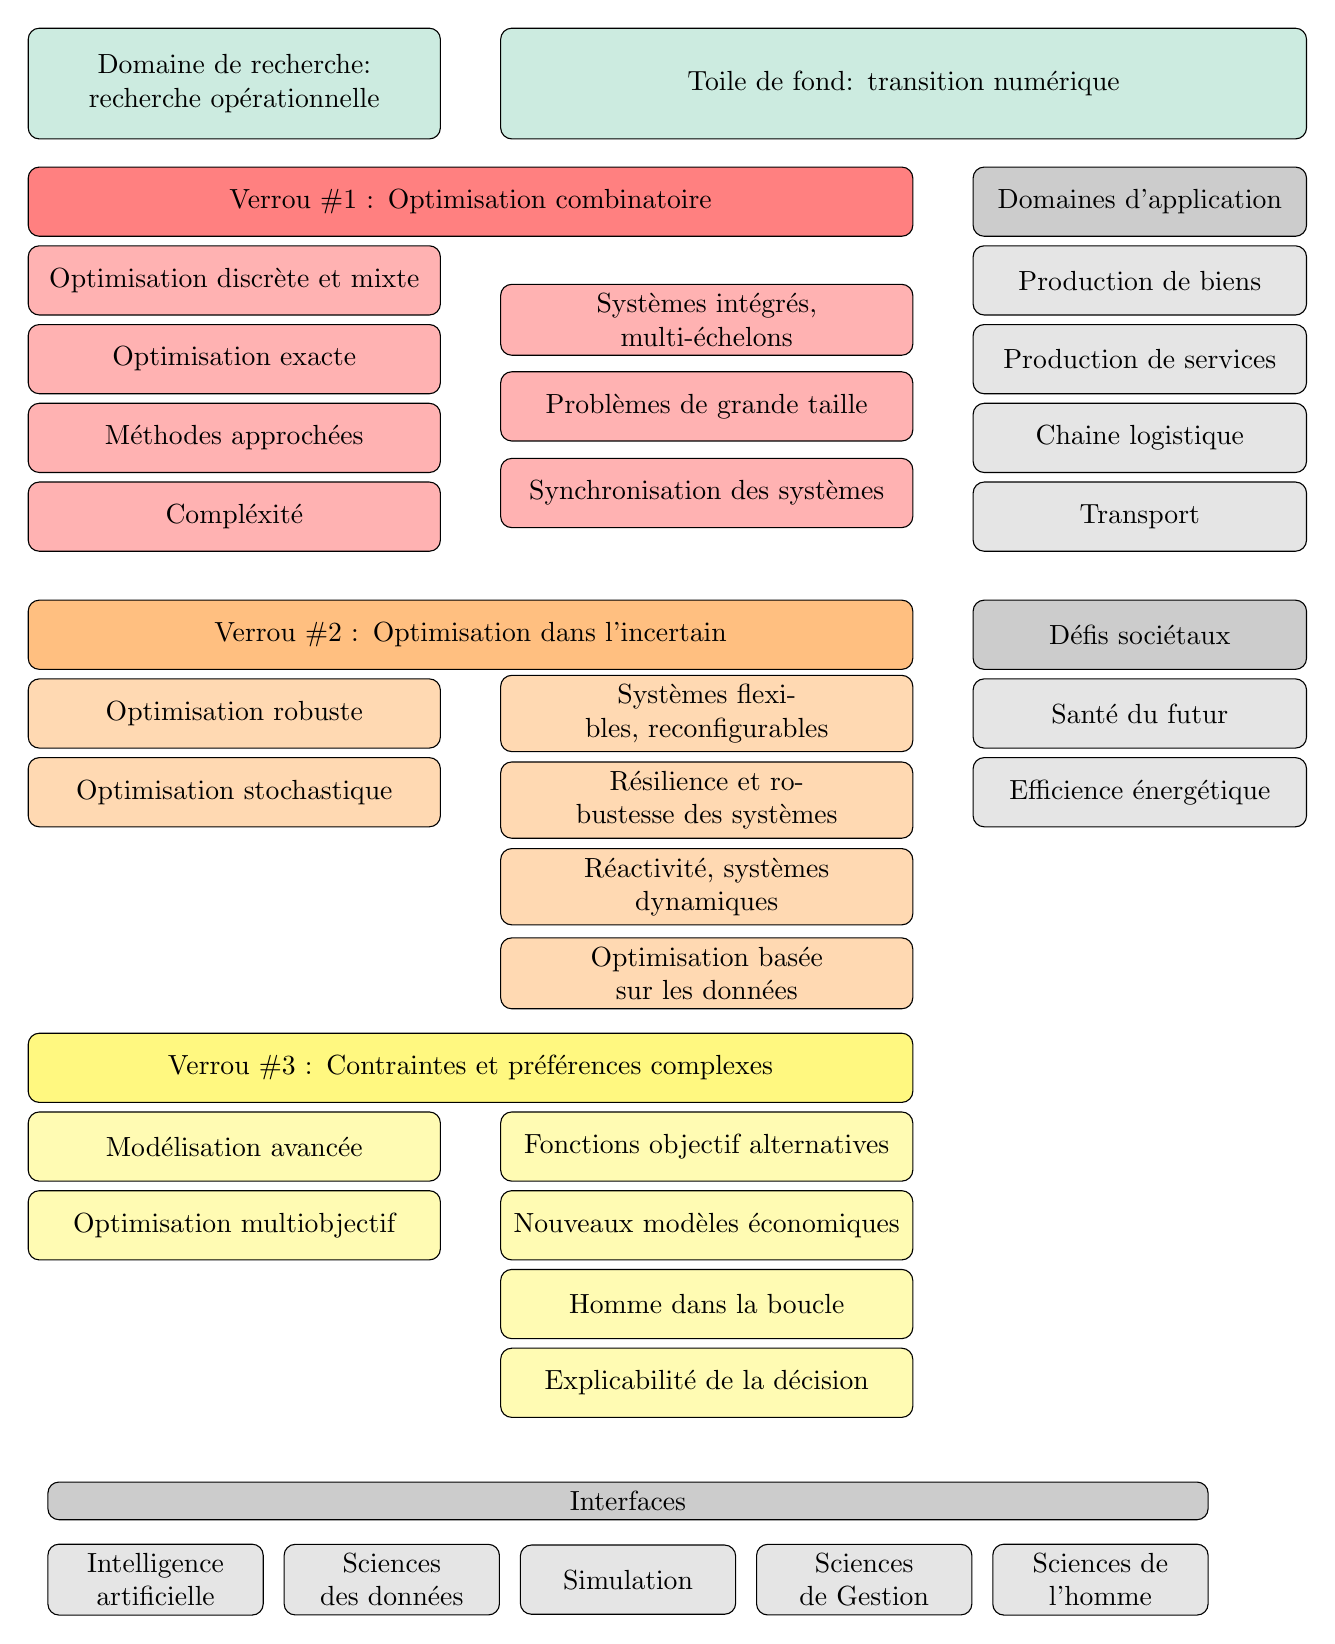
\begin{tikzpicture}[scale=0.5, auto]

    %  nodes  
    \node [chapeau, text width=5cm] (M) at (0,38) {Domaine de recherche: recherche opérationnelle};
    \node [chapeau, text width=10cm] (IF) at (17,38) {Toile de fond: transition numérique};
    
         
   %-------------------------------------------------------------
     \node[verrou, fill=red!50] at (6,35) {Verrou \#1 : Optimisation combinatoire};
    \node[detail1] at (0,33) {Optimisation discrète et mixte};
    \node[detail1] at (0,31) {Optimisation exacte};
    \node[detail1] at (0,29) {Méthodes approchées};
    \node[detail1] at (0,27) {Compléxité};
    
   \node[detail1] at (12,32) {Systèmes intégrés, multi-échelons};
   \node[detail1] at (12,29.8) {Problèmes de grande taille};
   \node[detail1] at (12,27.6) {Synchronisation des systèmes};

    
    %-----------------------------------------------------------
   \node[verrou, fill = orange!50] at (6,24) {Verrou \#2 : Optimisation dans l'incertain};     
   \node[detail2] at (0,22) {Optimisation robuste};
    \node[detail2] at (0,20) {Optimisation stochastique};
    
    \node[detail2] at (12,22) {Systèmes flexibles, reconfigurables};
    \node[detail2] at (12,19.8) {Résilience et robustesse des systèmes};
    \node[detail2] at (12,17.6) {Réactivité, systèmes dynamiques};
    \node[detail2] at (12,15.4) {Optimisation basée sur les données};

  
  %---------------------------------------------------------
     \node[verrou, fill=yellow!50] at (6,13) {Verrou \#3 : Contraintes et préférences complexes};

    \node[detail3] at (0,11) {Modélisation avancée};
    \node[detail3] at (0,9) {Optimisation multiobjectif};
    
    \node[detail3] at (12,11) {Fonctions objectif alternatives};
    \node[detail3] at (12,9) {Nouveaux modèles économiques};
    \node[detail3] at (12,7) {Homme dans la boucle};
    \node[detail3] at (12,5) {Explicabilité de la décision};
   
   
   %----------------------------------------------- 
   \node [detail, fill=gray!40] (D) at (23,35) {Domaines d'application};
    \node[detail] at (23,33) {Production de biens};
    \node[detail] at (23,31) {Production de services};
    \node[detail] at (23,29) {Chaine logistique};
    \node[detail] at (23,27) {Transport};

   \node [detail, fill=gray!40] (D) at (23,24) {Défis sociétaux};
    \node[detail] at (23,22) {Santé du futur};
    \node[detail] at (23,20) {Efficience énergétique};

     \node [chapeau2, text width=14.5cm] (I) at (10,2){Interfaces};
    \node[detail4] at (-2,0) {Intelligence artificielle};
    \node[detail4] at (4,0) {Sciences des données};
    \node[detail4] at (10,0) {Simulation};
    \node[detail4] at (16,0) {Sciences de Gestion};
    \node[detail4] at (22,0) {Sciences de l'homme};
    



  \end{tikzpicture}
  \caption{Détail du projet d'équipe}
  \end{figure}
  
  
		
		
		
		
		
		 
